\documentclass[border=6pt]{standalone}
\usepackage[T1]{fontenc}\usepackage{lmodern}\usepackage{amsmath,amssymb}\usepackage{graphicx}\usepackage{xcolor}\usepackage{tikz}
\usetikzlibrary{arrows.meta,positioning,calc,fit,shapes.misc,shapes.geometric}
% TikZ styles
\tikzset{
  blk/.style={draw, rounded corners=2pt, align=center, font=\small, minimum height=8mm, inner sep=4pt, fill=#1},
  blk/.default=white,
  arr/.style={-{Stealth[length=2.2mm]}, thick},
}
\definecolor{base}{HTML}{FBE3E3}
\definecolor{prop}{HTML}{DDEBFA}
\definecolor{same}{HTML}{EDEDED}
\definecolor{done}{HTML}{DFF1DF}
\definecolor{todo}{HTML}{FFF2CC}

\begin{document}
\begin{tikzpicture}[>=Stealth, font=\small,
  lab/.style={align=center, font=\footnotesize, text width=2.9cm},
  flow/.style={->, thick}]
  % (a) observation
  \node[inner sep=0pt, draw=gray!60] (obs) at (0,0) {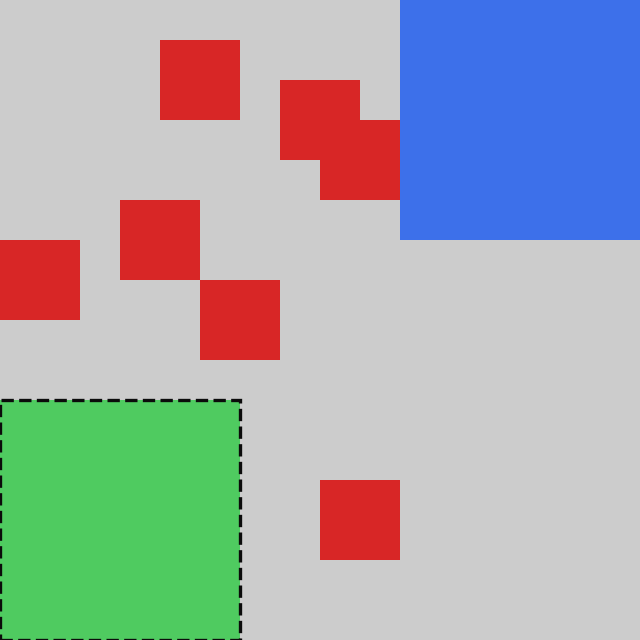
\includegraphics[width=2.3cm]{../routing_observation.png}};
  \node[lab, anchor=north] at (0,-1.45) {\textbf{(a) Observation}\\ health, droplet and goal channels};
  % (b) MC graph (4 x 3 excerpt)
  \begin{scope}[shift={(2.9,-0.7)}]
    \foreach \x in {0,...,3} \foreach \y in {0,...,2} {
      \ifnum\x<3 \draw[gray!60] (0.65*\x,0.7*\y) -- (0.65*\x+0.65,0.7*\y); \fi
      \ifnum\y<2 \draw[gray!60] (0.65*\x,0.7*\y) -- (0.65*\x,0.7*\y+0.7); \fi
      \ifnum\x<3 \ifnum\y<2
        \draw[gray!40] (0.65*\x,0.7*\y) -- (0.65*\x+0.65,0.7*\y+0.7);
        \draw[gray!40] (0.65*\x+0.65,0.7*\y) -- (0.65*\x,0.7*\y+0.7); \fi\fi }
    \foreach \x in {0,...,3} \foreach \y in {0,...,2}
      \node[circle, draw, fill=white, inner sep=0pt, minimum size=3.2mm] at (0.65*\x,0.7*\y) {};
    \foreach \p in {(0,0),(0.65,0)} \node[circle, draw, fill=blue!45, inner sep=0pt, minimum size=3.2mm] at \p {};
    \foreach \p in {(1.95,1.4),(1.3,1.4)} \node[circle, draw, fill=green!50!black!45, inner sep=0pt, minimum size=3.2mm] at \p {};
    \node[circle, draw, fill=red!55, inner sep=0pt, minimum size=3.2mm] at (1.3,0.7) {};
  \end{scope}
  \node[lab, anchor=north] at (3.875,-1.45) {\textbf{(b) MC graph}\\ $G=(V,E,X)$, 8-neighbour edges};
  % (c) three graph-convolution layers
  \foreach \i in {2,1,0}
    \draw[fill=prop, draw=blue!60!black, rounded corners=1.5pt] (6.3+0.2*\i,-0.95+0.2*\i) rectangle ++(1.7,1.5);
  \node[align=center, font=\footnotesize] at (7.15,-0.2) {GCN layer\\ $\times\,3$, $d=64$};
  \node[lab, anchor=north] at (7.35,-1.45) {\textbf{(c) Message passing}\\ $Z\in\mathbb{R}^{N\times 64}$};
  % (d) global max pooling: pooled vector
  \foreach \k/\s in {0/20,1/55,2/35,3/70,4/15,5/45,6/60,7/30}
    \draw[fill=blue!\s, draw=blue!60!black] (9.75,-0.95+0.24*\k) rectangle ++(0.34,0.24);
  \node[lab, anchor=north] at (9.92,-1.45) {\textbf{(d) Global max pooling}\\ $g\in\mathbb{R}^{64}$};
  % (e) PPO actor-critic
  \node[blk=same, minimum width=2.1cm] (actor) at (12.4,0.45) {Actor $\pi(a\,|\,s)$};
  \node[blk=same, minimum width=2.1cm] (critic) at (12.4,-0.55) {Critic $V(s)$};
  \node[lab, anchor=north] at (12.4,-1.45) {\textbf{(e) PPO}\\ actor--critic};
  % flow of the proposed pipeline
  \draw[flow] (1.25,0) -- (2.75,0);
  \draw[flow] (5.0,0) -- (6.2,0);
  \draw[flow] (8.5,0) -- (9.65,0);
  \draw[thick] (10.2,0) -- (10.6,0);
  \draw[flow] (10.6,0) -- (actor.west);
  \draw[flow] (10.6,0) -- (critic.west);
  \draw[flow] (actor.east) -- ++(1.1,0) node[right, font=\footnotesize, align=left] {action\\(1 of 8)};
  % baseline branch
  \node[blk=base, minimum width=5.6cm] (cnn) at (6.2,2.1) {Baseline encoder: CNN, 3 convolutional layers + FC};
  \draw[flow, dashed, red!60!black] (0,1.2) |- (cnn.west);
  \draw[thick, dashed, red!60!black] (cnn.east) -| (10.6,0);
\end{tikzpicture}
\end{document}
